\section{Propagation module}
\label{sec:propagation}
\begin{figure}[!h]
    \centering
    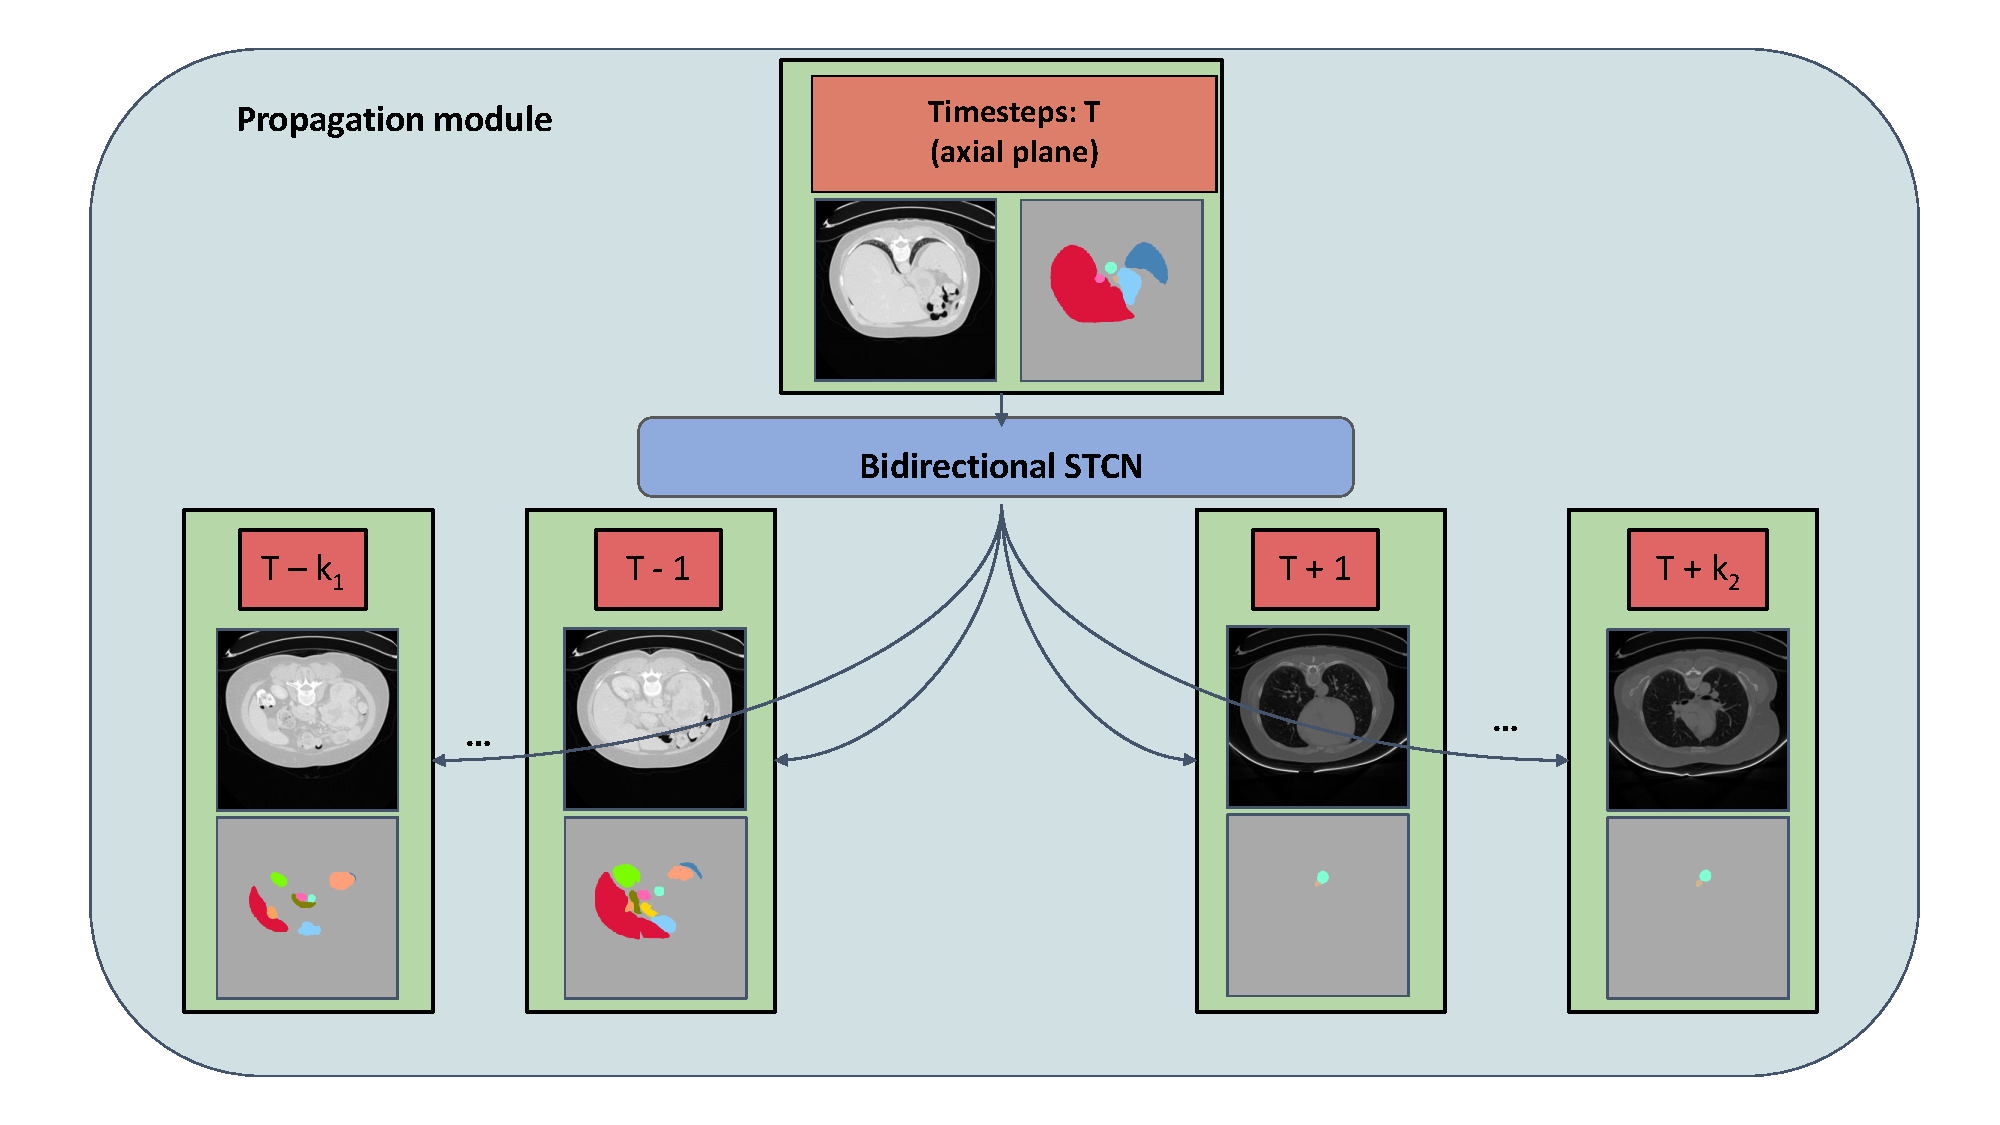
\includegraphics[width=\textwidth]{content/resources/new_images/propagation.pdf}
    \caption{The propagation module. From an annotated slice of CT, at timestep T, STCN can make use of that to spread the information through the entire defined range $[T-k_1, T+k_2]$.}
    \label{fig:propagation}
\end{figure}

This module aims to utilize prior knowledge of given annotated slices from the Reference module to make prediction on the remaining slices, this mechanism can be referred as mask (or label) propagation.

Intuitively, the conventional 2D CNNs cannot comprehend the third dimension information within a CT volume. Thus, in hope of the ability to capture the "temporal" information along the axial plane, we adapt the Space-Time Correspondence Networks (STCN) \cite{stcn21cheng}, which is a semi-supervised segmentation algorithm that has achieved promising results on Video object segmentation problem, to this 3D manner. 

Basically, STCN proposes the use of a memory bank that stores information about previous frames and their corresponding masks and uses them later as prior knowledge. To generate the mask for the current frame, a pairwise affinity matrix is calculated between the query frame and memory frames based on negative squared Euclidean distance, then it is used for supporting the current mask generation \cite{stcn21cheng}. 

Different from the original STCN, we slightly modify it to match the current problem. In the original work, they use only a single dense mask to propagate through the entire video, therefore for the model to perfectly work, that selected mask must contain information about all available classes. For our case to achieve that, we enable the usage of multiple masks for propagation, so that all of these masks should contain enough information about every organs. We also allow the STCN to work in a bidirectional way to enhance the refinement. Fig \ref{fig:propagation} illustrates this process.

Specially, STCN can be simply trained in the binary manner, meaning that each of the abdominal organs can be learned separately. Therefore, the knowledge can be transferred well between different organ classes.